\section[HO SiPM upgrade]{HO SiPM upgrade\footnote{Corresponding Author: Andreas K\"unsken}}\label{sec:hoSipmUpgrade}
\subsection{Hardware design}\label{kuenskenHardwareDesign}
In the first long shutdown of the LHC, HO was subject to upgrades. The previously used Hybrid Photo-Diodes (HPD) were replaced by SiPMs due to bad performance. The SiPM readout was designed as a drop-in replacement to keep most of the readout chain. The SiPMs were arranged on a newly produced Printed Circuit Board (PCB) to match the position of the pixels of the HPDs. The arrangement of the SiPMs is shown in Fig. \ref{kuenskensipmPcb}.
\begin{figure}[htbp]
\centering
\begin{minipage}[t]{0.475\textwidth}
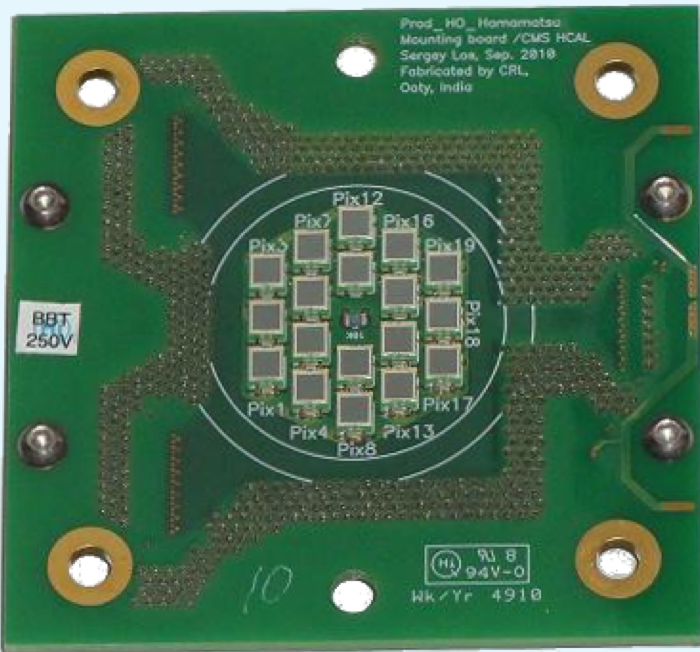
\includegraphics[width=\textwidth]{Figures/kuensken/pcbSipm.png}
\caption{PCB carrying 18 SiPMs. The white cirlce marks the position of the removed HPDs. Image adapted from \cite{beniCalor}.}
\label{kuenskensipmPcb}
\end{minipage}
\hspace{1cm}
\begin{minipage}[t]{0.435\textwidth}
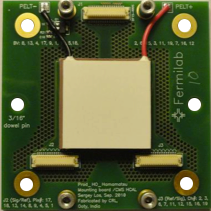
\includegraphics[width=\textwidth]{Figures/kuensken/pcbPeltier.png}
\caption{Backside of an HO PCB with the Peltier element attached. Image adapted from \cite{beniCalor}.}
\label{kuenskenpeltier}
\end{minipage}
\end{figure}
It can be seen that the new PCB has 18 SiPMs in the position where the 18 pixels of the HPDs were located.
The installed SiPM type was produced by Hamamatsu and is identical to a Hamamatsu S10931-050. It has an area of (3x3)\,mm$^2$ and comes with an SMD type housing. The cell pitch is 50\,$\mu$m.
Because HO has two layers of scintillator in ring 0 the number of fibers arriving at a single SiPM is larger in ring 0. As a consequence, the fibers cannot be arranged such that they completely fit inside the area of an SiPM. Therefore, a light mixer is installed between the ends of the fibers and the SiPM surface in ring 0. This light mixer
ensures that the light is distributed uniformly over the SiPM's surface, thus, avoiding the loss of light of only certain fibers.\\
SiPMs are solid state devices and rather sensitive to temperature changes, it is inevitable to provide a controlled temperature environment for a stable operation of the devices. A key feature is the change of the SiPM's breakdown voltage with temperature. The manufacturer specifies this quantity to 56\,$\frac{\text{mV}}{\text{K}}$. For this reason the PCBs carrying the SiPMs are equipped with Peltier elements on their backsides. Fig. \ref{kuenskenpeltier} shows a mounted Peltier element on a PCB.
\subsection{System performance}
\subsubsection{Temperature}
The performance of an SiPM changes strongly with the temperature if not corrected for. For this reason it is important to control the temperature of an SiPM before studying other parameters to make sure that any observed change is not due to a change in the temperature. Figure \ref{kuenskentemperatureStability} shows temperature deviations from a reference temperature plotted versus time.
\begin{figure}[htbp]
\centering
\begin{minipage}[t]{0.475\textwidth}
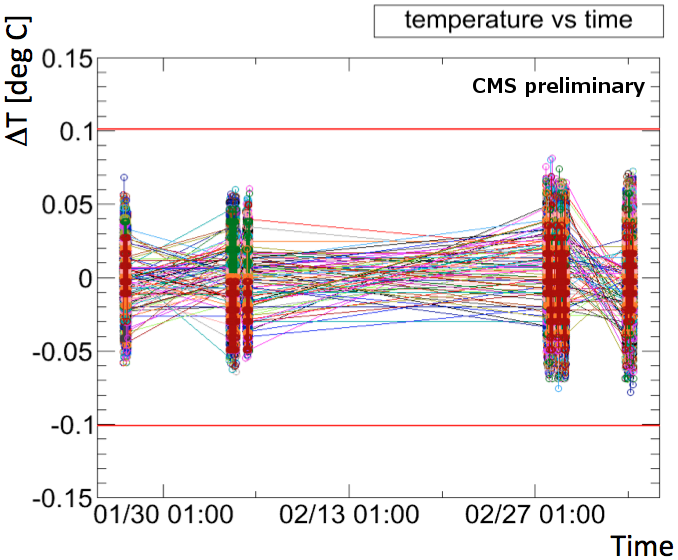
\includegraphics[width=\textwidth]{Figures/kuensken/temperature.png}
\caption{Fluctuation of temperature at the PCBs plotted versus time. The data points represent the temperatures at the PCBs for a given time. Fluctuations stay within 0.1\,$^\circ$C \cite{kuenskenCalor}.}
\label{kuenskentemperatureStability}
\end{minipage}
\hspace{0.5cm}
\begin{minipage}[t]{0.455\textwidth}
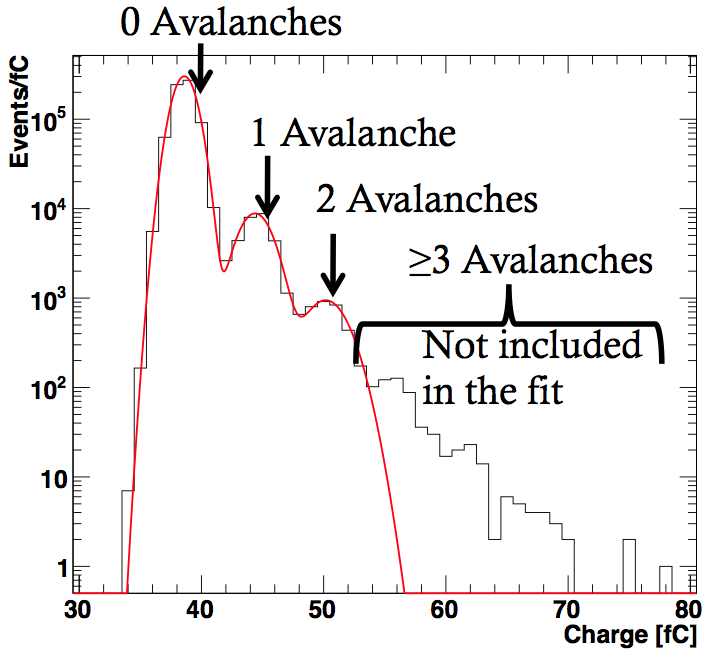
\includegraphics[width=\textwidth]{Figures/kuensken/gainDetermination.png}
\caption{Dark noise spectrum of an SiPM. plotted in red is the fit that is used for gain determination \cite{kuenskenCalor}.}
\label{kuenskendarkNoise}
\end{minipage}
\end{figure}
Each data point represents the temperature on a PCB at a given time. Deviations stay within a range of 0.1\,$^\circ$C which corresponds to a change of 5.6\,mV in the bias voltage.

\subsubsection{Gain}
The gain determines the signal height that is produced by an SiPM and thus the measured charge. It is necessary to know the gain of an SiPM to determine the number of photons that triggered the SiPM and get a measure of the deposited energy in the detector. HO uses two ways of determining the gain.
The first is to use the dark noise spectrum of an SiPM that develops due to thermal excitation of electrons in the active volume of an SiPM cell and the subsequent breakdown of that cell. A gauss fit is performed to the pedestal peak and the peaks of one and two avalanches. From the distance of the peak positions the gain is calculated. This method is known as the PED method. An example dark noise spectrum together with an applied fit is shown in Fig. \ref{kuenskendarkNoise}.
\begin{figure}[htbp]
\centering
\begin{minipage}[t]{0.475\textwidth}
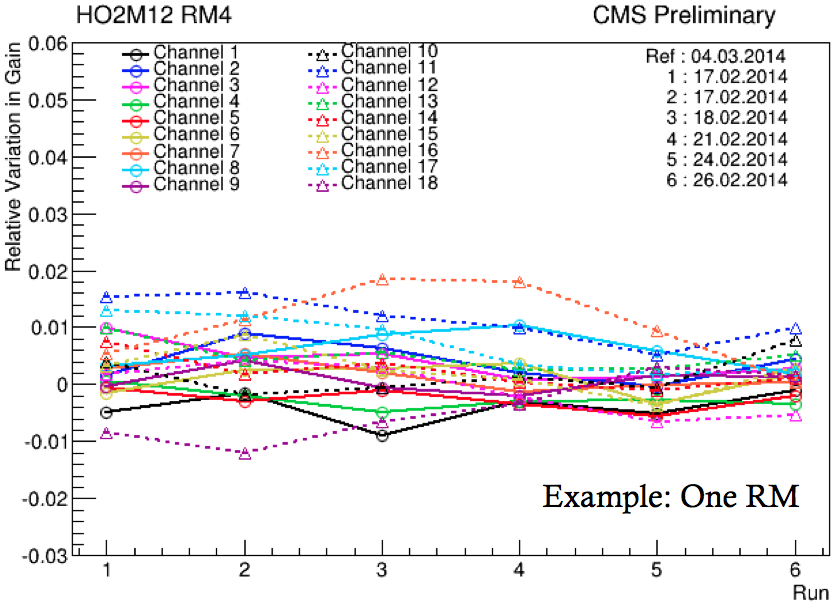
\includegraphics[width=\textwidth]{Figures/kuensken/gainOverTime.png}
\caption{Relative gain variation against time using the dark noise spectrum for gain determination \cite{kuenskenCalor}.}
\label{kuenskengainVsTime}
\end{minipage}
\hspace{0.5cm}
\begin{minipage}[t]{0.475\textwidth}
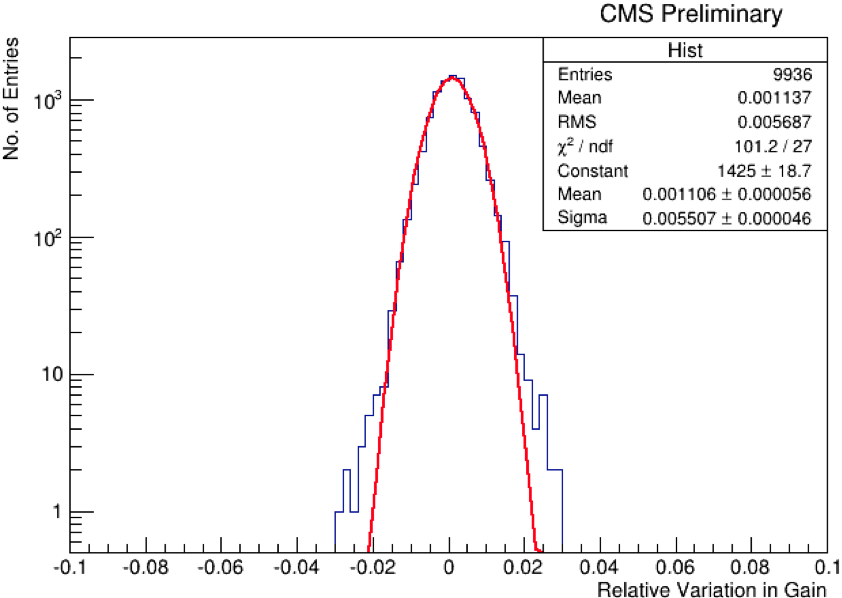
\includegraphics[width=\textwidth]{Figures/kuensken/gainTotal.png}
\caption{Histogram of all measured relative gain variations using the dark noise spectrum. The measurements were performed during the same period as is shown in Fig. \ref{kuenskengainVsTime} \cite{kuenskenCalor}.}
\label{kuenskengainHist}
\end{minipage}
\end{figure}
The second method uses short light pulses from an LED onto the SiPMs. When the light pulses contain not too many photons, the resulting signal distribution has a mean of
\begin{equation}
\text{m}=\text{N}\times \text{gain}
\end{equation}
and a width of
\begin{equation}
\sigma=\sqrt{\text{N}}\times \text{gain}
\end{equation}
assuming Poisson statistics for the uncertainty of the number of photons. Dividing the square of the measured width of the distribution by the measured mean, one obtains the gain of an SiPM as
\begin{equation}
\frac{\sigma^2}{\text{m}}=\frac{\text{N}\times \text{gain}^2}{\text{N}\times \text{gain}}=\text{gain.}
\end{equation}
This is called the LED method.
Before reviewing the comparability of the different methods it is necessesary to assure that the means of gain determination are stable. The relative gain variation versus time using the dark noise
spectrum is depicted in Fig. \ref{kuenskengainVsTime}. For a single PCB the relative gain variation is constant within 2\,\%. A histogram showing the relative gain variations for the same period for all installed SiPMs is plotted in Fig. \ref{kuenskengainHist}. The largest variations are within 3\,\%. The correlation between the two possibilities of determining the gain is printed in Fig. \ref{kuenskengainCorr}.
\begin{figure}[htbp]
\centering
\begin{minipage}[b]{0.475\textwidth}
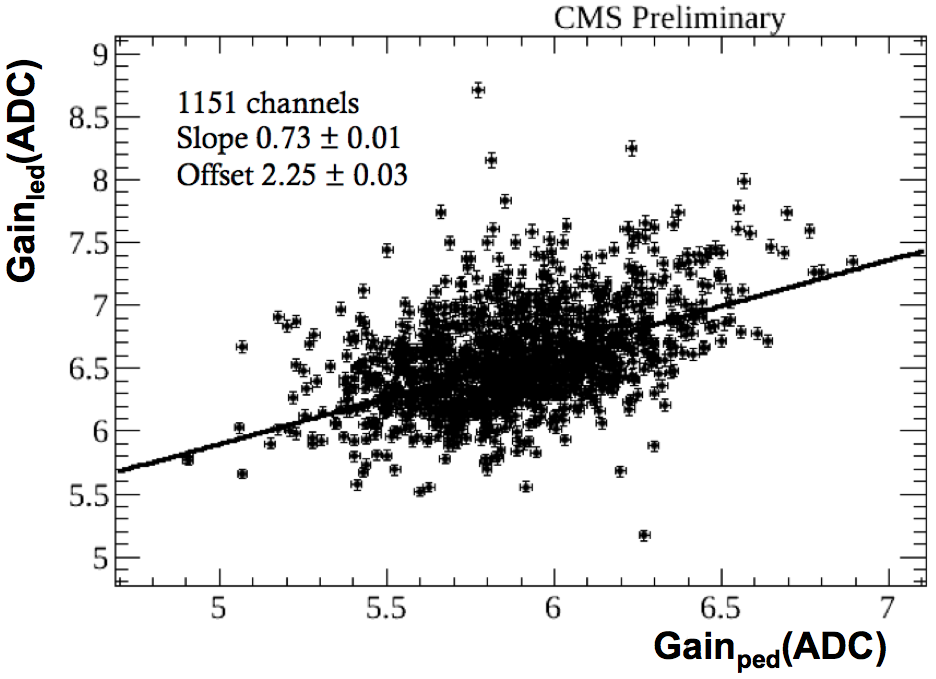
\includegraphics[width=\textwidth]{Figures/kuensken/gainCorrelation.png}
\end{minipage}
\hspace{0.5cm}
\begin{minipage}[b]{0.475\textwidth}
\caption{Correlation between the two methods for determining the gain. The values are distributed close to the design gain of 6\,ADC. Presented in \cite{kuenskenCalor}.}
\label{kuenskengainCorr}
\end{minipage}
\end{figure}
The plot shows that the measured gain values are centered around a specific value and no large deviation are found. However, it can be noticed that the mean gain value for the LED method is systematically shifted with respect to the results from the dark noise spectrum. This shift can be explained by the fact that the spectrum measured with the LED method is not exactly gaussian. This results in a shift towards higher gain values for this method. Once this offset has been characterized it would be possible to correct for it.

\subsubsection{Breakdown voltage}
The gain of an SiPM depends on the voltage difference between the applied voltage and the breakdown voltage of the device. It is therefore necessary to have reliable means of determining the breakdown voltage of an SiPM in order to keep the gain stable. In HO there are two ways of measuring the breakdown voltage. The first one exploits again the dark noise spectrum of an SiPM. By measuring the gain using the dark noise spectrum for different bias voltages the gain versus the bias voltage is plotted. It is then possible to fit a straight line to the distribution and extrapolate to a gain of zero pointing to the breakdown voltage. This is referred to as the PED method. The second way of breakdown voltage determination uses an LED again. The collected charge is measured for different bias voltages and then the relative derivative $\frac{\text{dS}}{\text{SdV}}$ is calculated. The resulting distribution has a maximum where the measured signal changes most with the bias voltage which is taken as the bias voltage. This method is referred to as the LED method.
\begin{figure}[htbp]
\centering
%\begin{minipage}[t]{0.475\textwidth}
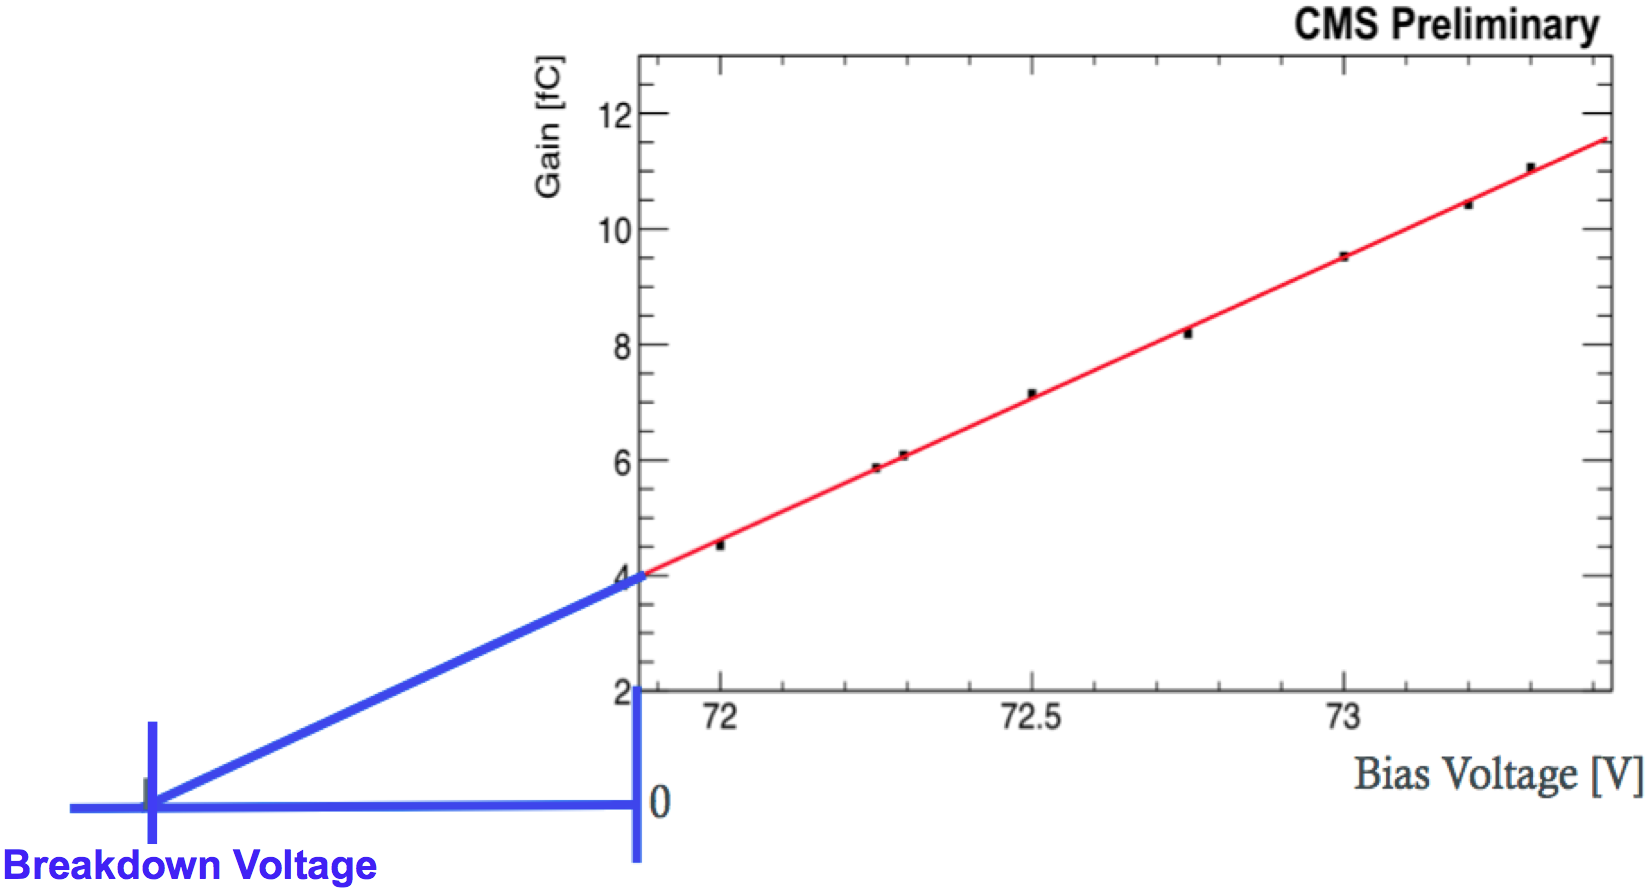
\includegraphics[width=0.9\textwidth]{Figures/kuensken/bvPedDetermination.png}
\caption{Determination of the breakdown voltage of an SiPM using the gain from dark noise spectrums measured at different bias voltages. Shown in \cite{kuenskenCalor}.}
\label{kuenskenbvPed}
%\end{minipage}
%\hspace{0.5cm}
\end{figure}
The determination of the breakdown voltage using the dark noise spectrum and the LED spectrum are shown in Fig. \ref{kuenskenbvPed} and Fig. \ref{kuenskenbvLed}, respectively.
\begin{figure}[htbp]
\centering
\begin{minipage}[htbp]{0.39\textwidth}
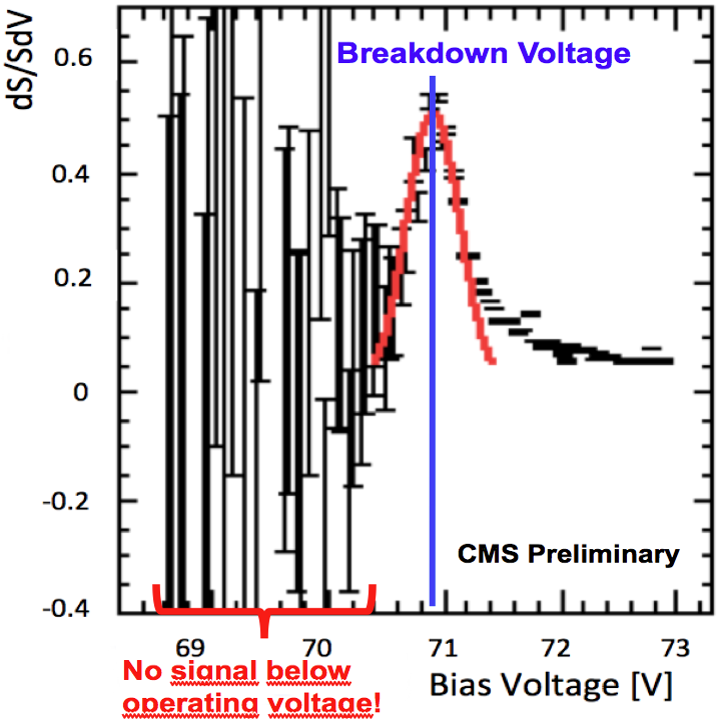
\includegraphics[width=\textwidth]{Figures/kuensken/bvLedScaled.png}
\caption{Breakdown voltage determination using the relative derivative of LED spectra measured at different bias voltages. Image from \cite{kuenskenCalor}.}
\label{kuenskenbvLed}
\end{minipage}
\hspace{0.5cm}
\begin{minipage}[htbp]{0.56\textwidth}
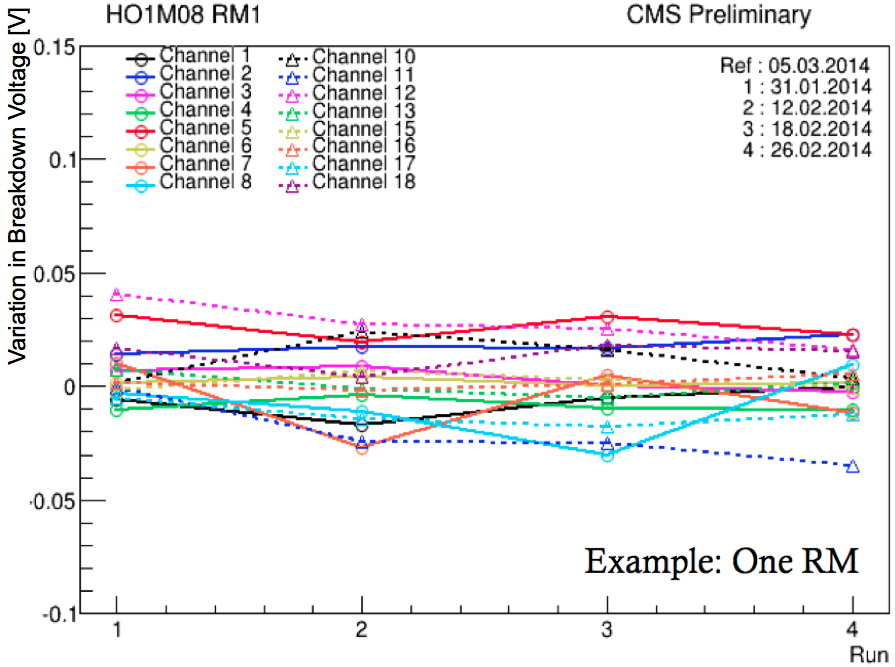
\includegraphics[width=\textwidth]{Figures/kuensken/bvOverTime.png}
\caption{Distribution of breakdown voltage measured with the PED method. Taken from \cite{kuenskenCalor}.}
\label{kuenskenbvVsTime}
\end{minipage}
\end{figure}
The variation of the breakdown voltage for a set of SiPMs on a single mounting board versus time is presented in Fig. \ref{kuenskenbvVsTime}. The employed method for the determination of the breakdown voltage is the PED method. The plot shows that the variation of the breakdown voltage stays within 50\,mV. The correlation between the two methods is shown in Fig. \ref{kuenskenbvCorr}. The data points align along a straight line which demonstrates a well defined linear relation between the values of the two methods. The spread of the breakdown voltages is due to the fact that not all devices have the same breakdown voltage. However, it can be noted that there is an offset between the two methods which shows itself in the y-intercept. This stems from the slightly different criteria for the determination of the breakdown voltage. Once the offset is determined the breakdown voltages can be corrected.
\begin{figure}
\centering
\begin{minipage}[htbp]{0.475\textwidth}
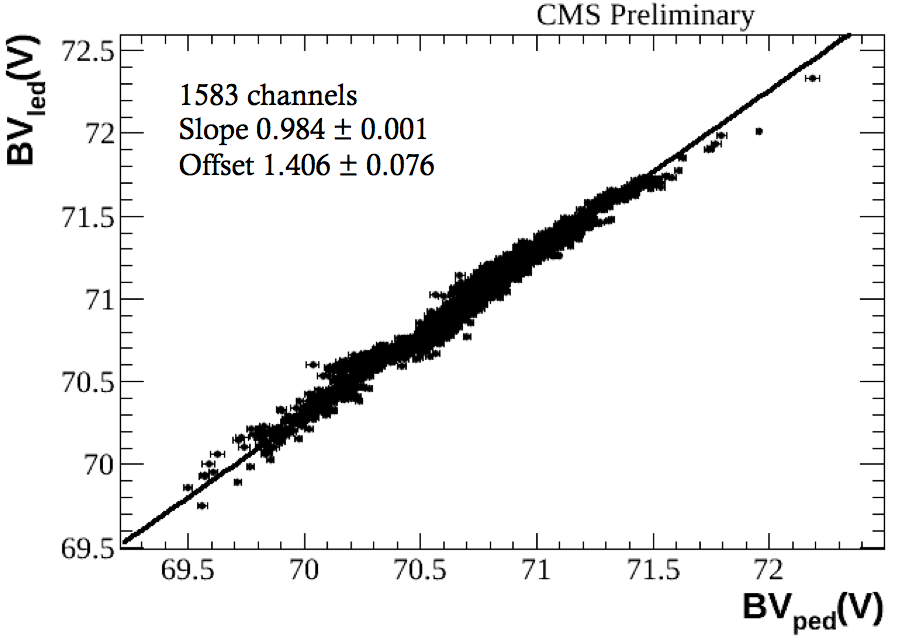
\includegraphics[width=\textwidth]{Figures/kuensken/bvCorrelation.png}
\end{minipage}
\hspace{0.5cm}
\begin{minipage}[htbp]{0.475\textwidth}
\caption{Correlation of the different methods for measuring the breakdown voltage. Taken from \cite{kuenskenCalor}.}
\label{kuenskenbvCorr}
\end{minipage}
\end{figure}
\newline
The HO system was successfully upgraded to SiPM readout during Long Shutdown 1, operation conditions (SiPM gain and breakdown voltage e.g.) are well understood and under control.
Studies on the muon detection capabilities of the already upgraded detector areas are now possible.